To generate all execution graphs that correspond to the given CGraph, we build one universal directed acyclic graph that includes all equivalent execution graphs and then extract them.

We build a universal graph iteratively.
In the first step, we add all environment sources to the universal graph and the sources list.
In the next one, we consider all available sources and operations, and if some sources satisfy input contracts of some operation, we add this operation to the universal graph and to the sources list.
The number of steps should be one more than the number of operations to ensure that the universal graph includes all graphs that correspond to the CGraph because, in this case, the longest possible path in the graph includes all available operations.

To extract all graphs corresponding to the CGraph, firstly, for each semantics node, we find all its occurrences in the universal graph.
Then we calculate a cartesian product of all these lists of occurrences.
Each element of the cartesian product includes occurrences of all semantics nodes.
For each such element, we extract an execution graph from the universal graph, which leaves are semantics nodes occurrences.
Finally, we filter graphs that do not have duplicated nodes.
These extracted graphs form a set of all equivalent graphs for the given task.

\begin{figure}
    \flushright
    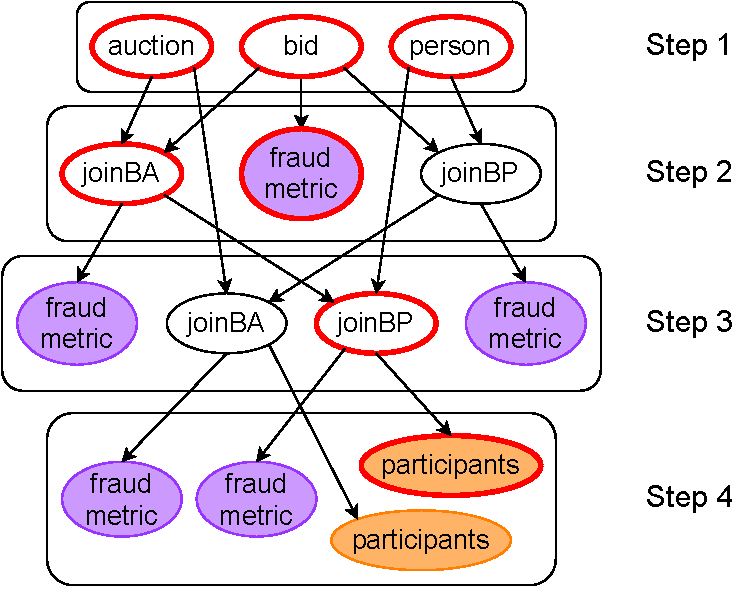
\includegraphics[width=0.4\textwidth]{images/generation}
    \caption{Generation of the running example graph.}
    \label{fig:gen}
\end{figure}

We use some tricks to make graphs generation faster.
Firstly, we keep a set of its predecessor operations for each source to filter the following operations (each execution graph cannot have node copies).
Secondly, we keep a set of the generated universal graph nodes to avoid adding the same nodes later.

% \begin{lstlisting}[language=Haskell]
% extract :: Graph -> Set NodeId -> Graph
% findIds :: Graph -> NodeName -> [NodeId]
% cartesianProduct :: [[a]] -> [[a]]

% semanticNids 
%   :: Graph -> Semantics -> [Set NodeId]
% semanticNids g = 
%     map Set.fromList . cartesianProduct 
%   . map (findIds g) . Set.toList

% genGraphs :: ( InCont s i, OutCont s o
%              , OutCont1 s o1, OutCont2 s o2) 
%           => CGraph i o o1 o2 -> [Graph]
% genGraphs (e, semantics) = 
%   let bigGraph = ... in
%   let graphs = 
%           map (bigGraph `extract`) 
%         $ semanticNids bigGraph semantics in
%   filter Graph.noSameNodes graphs
% \end{lstlisting}
